\documentclass[oneside,11pt]{amsart}
\usepackage[utf8]{inputenc}%
\usepackage[english]{babel}%
\usepackage{amsmath,amssymb,amsthm,amsfonts}%
\usepackage[unicode]{hyperref}%
\usepackage{mathrsfs,bbm}%
\usepackage{paralist}
\usepackage{color}
\usepackage{longtable}
\usepackage{array}
\usepackage{stmaryrd}%
%\usepackage{refcheck}
\usepackage{graphicx}
\usepackage[DIV15]{typearea}
\usepackage{multicol,tikz}
\usepackage{datetime}
\usepackage{cleveref}

\usepackage[shadow]{todonotes}

\usepackage{etoolbox}
\patchcmd{\section}{\scshape}{\large\itshape\bfseries}{}{}

\usepackage{caption}
\captionsetup{labelformat=empty,labelsep=none}

\hypersetup{
  colorlinks=true,
  linkcolor=blue!50!red,
  urlcolor=green!60!black
}

%%%%%%%%%%%%%%%%%%%%%%%%%%%%%%%%%%%%%%%%%%%%%%%%%%%%%%%%%%%%%%%%%%%%%%%%%%%%%%%%%%%%%%%%
\synctex=1
%%%%%%%%%%%%%%%%%%%%%%%%%%%%%%%%%%%%%%%%%%%%%%%%%%%%%%%%%%%%%%%%%%%%%%%%%%%%%%%%%%%%%%%%
%%%%%%%%%%%%%%%%%%%%%%%%%%%%%%%%%%%%%%%%%%%%%%%%%%%%%%%%%%%%%%%%%%%%%%%%%%%%%%%%%%%%%%%%

\begin{document}

\title[Building Truth from Scratch]{EGMT 1520: Building Truth from Scratch\\(Empirical \& Scientific Engagement)}
\author{Leonid Petrov\\Fall 2025}
\date{Compiled on \today, \currenttime. An up to date syllabus is always at \href{https://github.com/lenis2000/Syllabi/blob/master/Syllabus_EGMT_f25.pdf}{\texttt{this link}}.}
\maketitle


\section{How do we know a claim is true?}

This course is a hands-on workshop in making and testing arguments in the context of mathematics.
We will generate conjectures from examples, search for counterexamples, and turn ideas into precise statements and proofs. Through problem-solving sessions and math debates, you'll practice evaluating arguments, giving and receiving constructive feedback, and communicating clearly in writing and speech. By experiencing mathematics as a creative process --- where patterns suggest conjectures and logical reasoning turns intuition into conviction --- you'll develop a practical sense for what counts as evidence in mathematics and how to build reliable conclusions.
By the end of the course, you will be able to
\begin{enumerate}
    \item \textbf{Define and delimit what constitutes valid mathematical evidence} by distinguishing between examples, counterexamples, conjectures, and formal proofs, while recognizing the limitations of empirical observations.
    % \emph{(Aligned with pillar objective: “define and delimit what constitutes empirical evidence”)}
    \item \textbf{Develop a framework for discerning different types of mathematical knowledge} by exploring how empirical evidence, abstract reasoning, and logical structure work together to shape mathematical understanding.
    % \emph{(Aligned with pillar objective: “develop a framework for discerning types of knowledge based on what is empirically
% observable in the natural, physical and social worlds”)}
    \item \textbf{Formulate and communicate mathematical reasoning} by translating intuitive insights into precise statements, evaluating the soundness of arguments, and engaging in constructive dialogue to identify and resolve reasoning gaps.
    % \emph{(Aligned with pillar objective: “evaluate supported claims about the natural and social worlds by framing empirical questions and methods and interpreting the claims in the context of new data”)}
    \item \textbf{Reflect on the nature of mathematical truth} by examining personal assumptions about certainty, analyzing when and why certain arguments are conclusive, and articulating how purely empirical approaches can both inform and limit our understanding of complex phenomena.
    % \emph{(Aligned with pillar objective: “articulate the limitations of using only empirical approaches to describe complex phenomena”)}
\end{enumerate}


\begin{center}
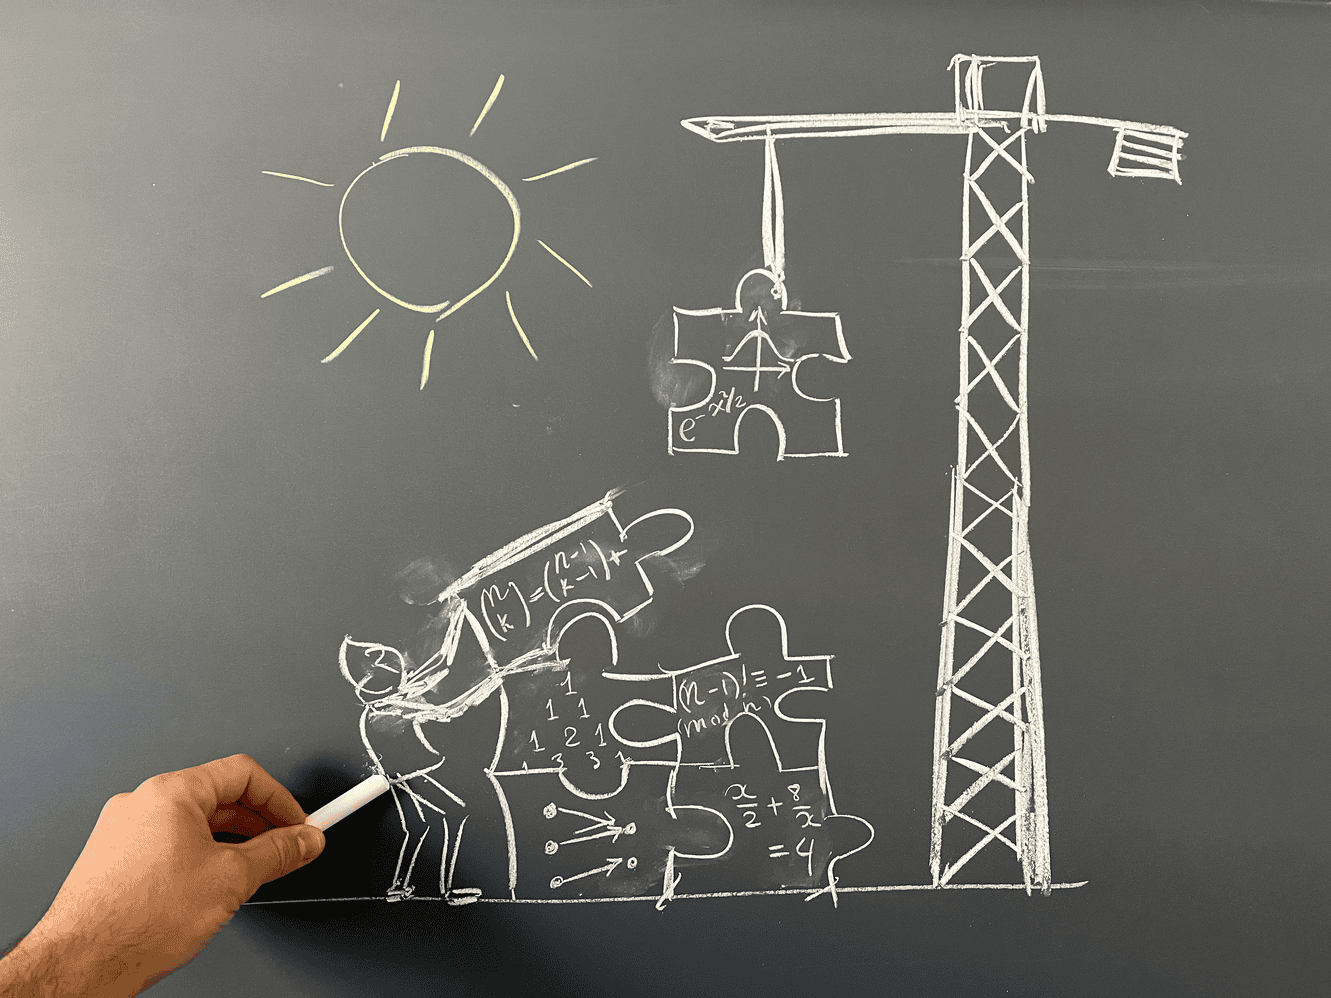
\includegraphics[width=.5\textwidth]{EGMT_image.png}
\end{center}

\newpage
\section{Contact \& Logistics}

\noindent
\begin{tabular}{ll}
\textbf{Instructor:} Leonid Petrov &\qquad \qquad \qquad\textbf{Office:} 209 Kerchof Hall \\
\textbf{Email:} \href{mailto:petrov@virginia.edu}{petrov@virginia.edu} & \qquad \qquad \qquad\textbf{Office hours:} TBA. \\
\end{tabular}

\vspace{4pt}

\noindent\textbf{Meetings:} 
Mondays 3:30--6:00PM, Gilmer Hall 247
(September 1, 8, 15, 22, 29; October 6).

\medskip
\noindent
\textbf{Math debate split session:} One additional session of math debates in the weeks of September 15 and 22. 
Class split in half by poll (others welcome to attend the debate, too).

\section{How we work together}

we work on problem sets 

these problem sets are not requiring any math knowledge beyond middle school, but go in a different direction that many student might not be familiar with (if you have a background, make sure to not put more than one such person in a group)

you see a new problem set when coming to class

during class you discuss with the group the problems and the group presents them orally when ready

I try to find counterexamples and be competitive about your solution (be ready to defend your solution)

when in presentation, I can ask another subgroup member to continue the presentation at any moment, so before presenting, make sure that all group members undertand all the details of the solution

we will also have mixers during each class for shared experience and to get to know each other better


also, starting from second class, we will have mini-debates: one person presents a problem, other subgroups work on counterexamples and finding holes in the argument, or asking questions




this is a pen and paper course, no devices are allowed during class


common place book is good for taking notes, but scrap ppaer will also be available. 

we sometimes will use manipulatives


\begin{enumerate}[$\bullet$]
  \item \textbf{Subgroups:} At the first meeting, we form 6 fixed ``home subgroups'' 
	for collaboration during class meetings. 

	Subgroups are
	$\delta, \ \theta, \ \zeta, \ \sigma, \ \lambda, \ \phi$

	for trust, momentum, and shared notation. Most meetings include a 10-minute \emph{random mixer} to cross-pollinate ideas.
  \item \textbf{Debates:} Frequent \emph{mini-debates}, one \emph{Big Debate Meeting}, and a \emph{Final Showcase}. On-stage teams never exceed 8 speakers; non-speakers serve as analysts, question writers, and judges.

  \item \textbf{Studio norm:} Keep devices in your bag during activities (think: yoga studio / lab). Accessibility accommodations always honored.
  \item \textbf{Commonplace book:} Your paper notebook for pre-class recaps, in-class sketches, diagrams, drafts, and reflections.
\end{enumerate}


\section{Assignments and grading}

(put percentages here)

assignments :

- presenting problems during class
- commonplace book: problem write ups (submti to canvas)
- debates
- engaging grounds
- final reflection short essay (2 pages) ``what counts as evidence in mathematics?''

Final reflection due after the last class (on Friday the week of October 6).

\section{What to bring each time}
scrap paper; pen/pencil; your commonplace book.

curiosity


Collaboration welcome during class and on homework, but write up your own solutions.







\section{Policies (brief)}


USE of AI: not for class; okay for learning during homework, but not for writing up solutions.
this is a prompt for learning: \url{https://gist.githubusercontent.com/lenis2000/cb5ea004f8aa6461be71398e19ae488e/raw/a0103eab0b865a1cedf2f3bf3c00d217bd294005/AI_hint_prompt.txt}

During in-class activities and debates, use analog materials unless your accommodation specifies otherwise.

(add details from usual syllabus)


SDAC letters are welcome; please share early so we can plan. The UVA Honor System applies to all work. If you hit academic or personal turbulence, reach out---earlier is better.

\textbf{Attendance \& grade scale:} Engagements policies on Canvas apply.\\
\textbf{Deadlines:} Because work builds on discussion, due dates matter; contact me early if a conflict looms.\\
\textbf{Devices:} Off and away during activities (unless accommodated).\\
\textbf{Honor:} Cite collaborators/tools; write your own text.

\end{document}
